\subsection{Permutation and Randomization Tests}

\datum{Lecture 7: 01/27}
\emph{\textbf{Goal.}} We want a strategy to compute a p-value for testing a hypothesis when we do no trust / want to assume a parametric model that would give a closed-form null distribution. We do this by recomputing a test statistic under transformation of the observed data that are valid under $H_0$.

Let $T\colon \textup{data} \rightarrow \mathbb{R}$ with larger $T$ iff there is more evidence against $H_0$. Write $T_{\textup{obs}} := T(\textup{observed data})$ for the observed value of the test statistic. For example, for testing independence with real-valued, one can define $T:= | \textup{Sample Correlation}|$. 

If we assume a parametric model, we might compute the null distribution of $T$ analytically. Without this assumption, we approximate the null distribution by
\begin{itemize}
    \item \emph{\textbf{Randomization Test.}} Generate synthetic datasets from a null distribution and recompute T.
    \item \emph{\textbf{Permutation Test.}} Generate new datasets by permuting labels/indices in a way that is valid under $H_0$ and recompute T.
\end{itemize}

\begin{example}
    We observe i.i.d. pairs $(X_i,Y_i)$ for $i\in[n]$ and want to test independence
    $$
    H_0 \colon X \perp Y \quad \textup{or equivalently }(X,Y)\sim P_X \times P_Y \quad \textup{vs.} \quad H_1 \colon X\not\perp Y.
    $$

    Let $T((X_1,Y_1),\dots,(X_n,Y_n))$ be a test statistic like sample correlation. The question is how to generate $\hat{T}_1, \dots, \hat{T}_m$ representing what $T$ would look like under $H_0$.

    \begin{itemize}
        \item[\textbf{Case 1:}] We know both marginals $P_X$ and $P_Y$. Then $$H_0\colon (X_i, Y_i)\stackrel{i.i.d.}{\sim} P_X\times P_Y$$ and we can simulate i.i.d. null datasets $(\Tilde{X}_1^{(m)}, \Tilde{Y}_1^{(m)}), \dots, (\Tilde{X}_m^{(m)}, \Tilde{Y}_m^{(m)}) \stackrel{i.i.d.}{\sim} P_X\times P_Y$ for $m=1,\dots, M$ and compute $\hat{T}_m = T\left((\Tilde{X}_1^{(m)}, \Tilde{Y}_1^{(m)}), \dots, (\Tilde{X}_m^{(m)}, \Tilde{Y}_m^{(m)})\right)$. Under $H_0$ $$T, \hat{T}_1,\dots, \hat{T}_M \textup{ are i.i.d from the null distribution.}$$

        \item[\textbf{Case 2:}] We know one marginal (say $P_X$) but not $P_Y$. Then $$H_0\colon (X_i, Y_i)\stackrel{i.i.d.}{\sim} P_X\times P_Y \quad \textup{for some unkown }P_Y.$$ Under $H_0$ $$(T, \hat{T}_1,\dots, \hat{T}_M) \mid (Y_1,\dots,Y_n) \textup{ are i.i.d from the null distribution of T} \mid  (Y_1,\dots,Y_n).$$

        \item[\textbf{Case 3:}] We do not know either marginal. We assume that under $H_0$ the pairs are i.i.d. from $P_X\times P_Y$ for some $P_X,P_Y$. A permutation test generates null datasets by breaking the paring between $X$ and $Y$. 

        Let $\pi_m$ be a random permutation of $[n]$, then define $\Tilde{T}_m := T\left((X_{\pi_m(1)}, Y_1),\dots, (X_{\pi_m(n)}, Y_n)  \right)$. One can also permute $Y$ instead of $X$ or apply permutations to both $X$ and $Y$. Under $H_0$ $$(T, \hat{T}_1,\dots, \hat{T}_M) \mid (Y_1,\dots,Y_n) , (Y_1,\dots,Y_n) \textup{ are i.i.d from the conditional null distribution of T}.$$
    \end{itemize}

\begin{figure}[h!]
    \centering
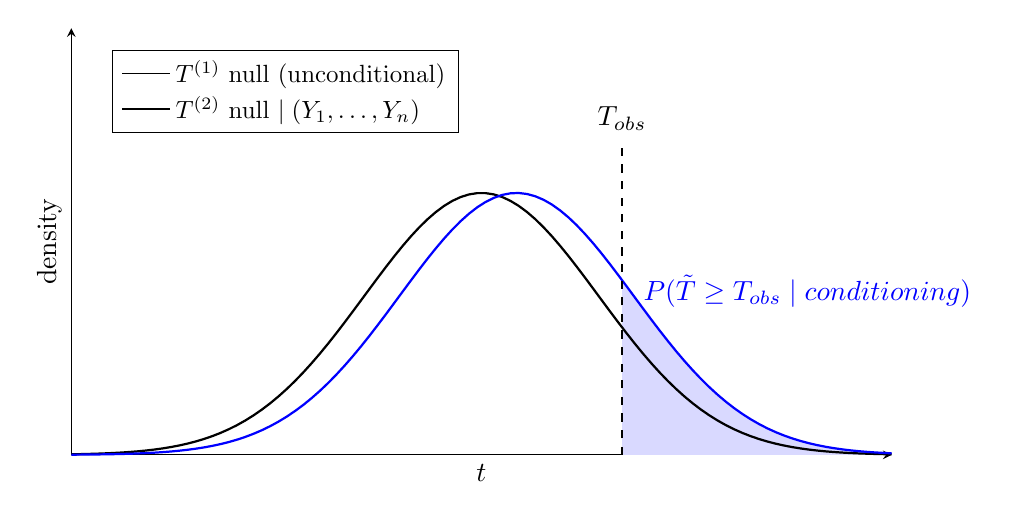
\begin{tikzpicture}
    \begin{axis}[
        % Axis setup
        axis lines = left,
        xlabel = $t$,
        ylabel = {density},
        ymin=0, ymax=0.65,
        xmin=-3.5, xmax=3.5,
        ticks=none, % Hide numeric ticks to match style
        clip=false, % Allow labels to extend beyond axis
        width=12cm,
        height=7cm,
        % Legend setup
        legend style={
            at={(0.05,0.95)}, 
            anchor=north west, 
            nodes={scale=0.9, transform shape},
            draw=black
        },
        legend cell align={left}
    ]

    % Define parameters for the distributions
    \def\muBlack{0}
    \def\sigmaBlack{1}
    \def\muBlue{0.3} % Slightly shifted to the right
    \def\sigmaBlue{1}
    \def\Tobs{1.2}   % The observed T value

    % Gaussian formulas
    \def\gaussBlack{1/(\sigmaBlack*sqrt(2*pi))*exp(-((x-\muBlack)^2)/(2*\sigmaBlack^2))}
    \def\gaussBlue{1/(\sigmaBlue*sqrt(2*pi))*exp(-((x-\muBlue)^2)/(2*\sigmaBlue^2))}

    % 1. Shaded Region (Draw this first so it is behind the lines)
    % Area under the BLUE curve starting from T_obs
    \addplot [
        fill=blue!15,
        draw=none,
        domain=\Tobs:3.5,
        samples=50
    ] {\gaussBlue} \closedcycle;

    % 2. Black Curve (Unconditional Null)
    \addplot [
        thick,
        black,
        domain=-3.5:3.5,
        samples=100
    ] {\gaussBlack};
    \addlegendentry{$T^{(1)}$ null (unconditional)}

    % 3. Blue Curve (Conditional Null)
    \addplot [
        thick,
        blue,
        domain=-3.5:3.5,
        samples=100
    ] {\gaussBlue};
    \addlegendentry{$T^{(2)}$ null $\mid (Y_1,\dots,Y_n)$}

    % 4. Vertical Dashed Line at T_obs
    \draw [dashed, semithick] (axis cs:\Tobs, 0) -- (axis cs:\Tobs, 0.48);

    % 5. Annotations
    % T_obs label
    \node at (axis cs:\Tobs, 0.48) [above] {$T_{\text{obs}}$};
    
    % Probability label (blue text)
    \node[blue, anchor=west] at (axis cs: \Tobs + 0.1, 0.25) {$\mathbb{P}(\tilde{T} \geq T_{\text{obs}} \mid \text{conditioning})$};
    \end{axis}
\end{tikzpicture}
\end{figure}

Null distributions for a test statistic $T$ and the right-tail $p$-value. The shaded region is the right-tail probability beyond the observed value $T_{\text{obs}}$, which is estimated by $p = \frac{1 + \#\{m: \tilde{T}_m \ge T_{\text{obs}}\}}{M+1}$. 
\end{example}

In each case (1)-(3), the construction ensures that under $H_0$ the collection
$$(T, \hat{T}_1, \dots, \hat{T}_m)$$
is exchangeable.

\begin{defn}[Exchangeability]
Random variables $Z_1,\dots, Z_K$ are \emph{exchangeable} if
$$
(Z_1,\dots,Z_K) \stackrel{d}{=} (Z_{\pi_1}, \dots, Z_{\pi_K}) \quad \textup{for every permutation } \pi \textup{ of } [n].
$$
\end{defn}

\emph{\textbf{Note.}} (Conditional) Independence implies (conditional) exchangeability.

Given $M$ null replicates $\hat{T}_1, \dots, \hat{T}_M$, define the p-value

\begin{equation}
p = \frac{1+\sum_{m=1}^M\mathbbm{1}_{\hat{T}_m \geq T_{\textup{obs}}}}{M+1}
\end{equation}

Let $k$ be the position of $T_{\text{obs}}$ in the sorted list of the $M + 1$ values $\{T_{\text{obs}}, \tilde{T}_1, \dots, \tilde{T}_M\}$ ordered from high to low. If there are no ties, then exactly $k - 1$ of the $\tilde{T}_m$'s exceed $T_{\text{obs}}$, so
\[
\#\{m : \tilde{T}_m \ge T_{\text{obs}}\} = k - 1
\]
and therefore
\[
p = \frac{1 + \#\{m : \tilde{T}_m \ge T_{\text{obs}}\}}{M+1} = \frac{1 + (k - 1)}{M+1} = \frac{k}{M+1}.
\]
By exchangeability under $H_0$, the rank $k$ is uniform on $\{1, \dots, M + 1\}$, implying $p$ is super-uniform.

\begin{thm}{Exchangeability and super-uniformity}{Exchangeability and super-uniformity}
    If $(T, \hat{T}_1,\dots,\hat{T}_M)$ are exchangeable under $H_0$, then $p$ is super-uniform under $H_0$ 
    \begin{align*}
        \mathbb{P}[p\leq \alpha] \leq \alpha \quad \textup{for all } \alpha \in [0,1] 
    \end{align*}
\end{thm}
\begin{pr}
    (\textbf{Idea}) Assume for simplicity there are no ties among $T_{\textup{obs}}, \Tilde{T}_1, \dots, \Tilde{T}_m$. Then $p$ as in (1) is a deterministic function of the rank of $T$ and exchangeability implies that the rank is uniform on $\{1,\dots, M+1\}$, which implies super-uniformity.
\end{pr}

Small $M$ is fine for validity (super-uniformity still holds). It mainly affects power/resolution: the $p$-value cannot be smaller than $1/(M + 1)$, so very small $p$-values require larger $M$. The main technical challenge in applications is verifying exchangeability (i.e., choosing a shuffling/resampling scheme that is valid under $H_0$).